\documentclass{beamer}
\usepackage{etex}
\usepackage{tabularx}
\usepackage[spanish,activeacute]{babel}
\usepackage[utf8]{inputenc}
\usepackage{graphics}
\usepackage{url}
\usepackage{ulem}
\usepackage{beamerthemesplit}
\usepackage{hyperref}
\usepackage{wrapfig}
\usepackage{listings}
\usepackage{color}
\usepackage{adjustbox}
\usepackage{multicol}
\usepackage{slashbox,pict2e}
\usepackage{tikz}
\usetikzlibrary{shapes,arrows}

\usepackage{algorithm}
\usepackage{algorithmic}
\renewcommand{\algorithmicrequire}{\textbf{Input:}}
\renewcommand{\algorithmicensure}{\textbf{Output:}}

\usetheme{CambridgeUS}
\usecolortheme{seahorse}

\makeatother
\setbeamertemplate{footline}
{
  \leavevmode%
  \hbox{%
  \begin{beamercolorbox}[wd=.4\paperwidth,ht=2.25ex,dp=1ex,center]{author in head/foot}%
    \usebeamerfont{author in head/foot}Jonathan Antognini, Luis Salinas, Paola Arce%\insertshortauthor
  \end{beamercolorbox}%
  \begin{beamercolorbox}[wd=.6\paperwidth,ht=2.25ex,dp=1ex,center]{title in head/foot}%
    \usebeamerfont{title in head/foot}\insertshorttitle\hspace*{3em}
    \insertframenumber{} / \inserttotalframenumber\hspace*{1ex}
  \end{beamercolorbox}}%
  \vskip0pt%
}
\makeatletter
\setbeamertemplate{navigation symbols}{}

\usepackage{pstricks}
\usepackage{multicol}

\tikzstyle{startstop} = [rectangle, rounded corners, minimum width=3cm, minimum height=1cm,text centered, draw=black, fill=red!30]
\tikzstyle{io} = [trapezium, trapezium left angle=70, trapezium right angle=110, minimum width=3cm, minimum height=1cm, text centered, draw=black, fill=blue!30]
\tikzstyle{process} = [rectangle, minimum width=4cm, minimum height=1cm, text centered, text width=5cm, draw=black, fill=orange!30]
\tikzstyle{decision} = [diamond, minimum width=2cm, minimum height=1cm, text centered, draw=black, fill=green!30]
\tikzstyle{arrow} = [thick,->,>=stealth]



\title{High-Frequency Trading \\ \& \\ Graphics Processing Unit}
\subtitle{Examen de Titulación}
\author{Jonathan Antognini C.\\
		Prof. Guía Dr. Luis Salinas\\
        Prof. Correferente M.Sc Paola Arce}
\institute[UTFSM]{Universidad Técnica Federico Santa María}
\date{\today}

\begin{document}
    \AtBeginSection[]
    {
      \begin{frame}
        \frametitle{Tabla de contenidos}
        \begin{multicols}{2}
        \tableofcontents[currentsection]
        \end{multicols}
      \end{frame}
    }

    \frame{\titlepage}
    \begin{frame}{\contentsname}
        \frametitle{Tabla de Contenidos} 
        \begin{multicols}{2}
        \tableofcontents
        \end{multicols}
    \end{frame}

    \section{Objetivos}
        \begin{frame}
            \frametitle{Objetivos de la memoria}
            \noindent Los \emph{\textbf{objetivos principales}} de esta memoria son:
            \begin{itemize}
             \item Implementar un modelo VEC y analizar su comportamiento con
            series financieras de alta frecuencia.
             \item Optimizar dichos algoritmos usando computación de alto desempeño
            (GPU) para mejorar su rendimiento.
            \end{itemize}
            
            \noindent Los \emph{\textbf{objetivos secundarios}}:
            \begin{itemize}
                \item Adaptar el modelo VEC para este tipo serie, encontrando
            los parámetros apropiados para su funcionamiento.
                \item Evaluar la factibilidad de optimizar el modelo VEC mediante la
            programación de alto desempeño (GPU).
            \end{itemize}

        \end{frame}

    \section{Introducción}
        \subsection{Mercados Financieros}
            \begin{frame}
            \frametitle{Mercados Financieros}
                El mercado financiero es un espacio con marco institucional que
                permite poner en contacto a oferentes y demandantes para que efectúen
                transacciones financieras. Terminología:
                \begin{itemize}
                    \item \emph{Dealer}
                    \item \emph{Orders}
                    \item \emph{Bid price}
                    \item \emph{Ask price}
                    %\item \emph{Market orders}
                    %\item \emph{Limit orders}
                \end{itemize}
            \end{frame}
        \subsection{Serie de tiempo Forex}
            \begin{frame}
            \frametitle{Serie de tiempo Forex}
            Una tendencia en el análisis de las series financieras, es el seguimiento del
            precio de un instrumento en el tiempo.
            \begin{figure}[h!t]
                \begin{center}
                    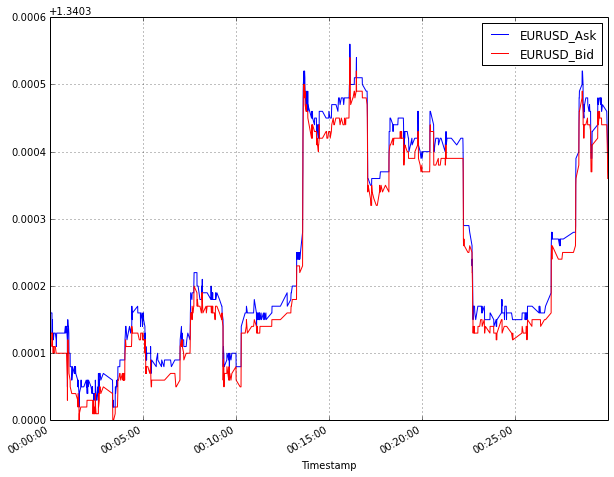
\includegraphics[width=0.5\textwidth]{img/eurusd}
                    \caption{Serie de tiempo EURUSD}
                    \label{fig:microsoft}
                \end{center}
            \end{figure}

            \end{frame}
    \section{Descripción del problema}
        \subsection{Series de tiempo estacionarias}
            \begin{frame}
            \frametitle{Series de tiempo estacionaria}
            Una serie de tiempo $\{y_{t_n}\}, n \in \mathbf{Z}$ se dice estrictamente
            estacionaria cuando el comportamiento probabilístico de cada colección
            correlativa de valores $\{y_{t_1},y_{t_2},\dots,y_{t_L}\}$ es idéntico a otro
            set correlativo desplazado en el tiempo:
            \[ P\{y_{t_1} \leq
            c_1,\dots,y_{t_L} \leq c_L\} = P\{y_{t_1+h} \leq c_1,\dots,y_{t_L+h}
            \leq c_L\}
            \quad \forall L \in \mathbb{N}, \forall h \in \mathbb{Z}\] \noindent donde
            $c_1,\dots,c_L$ son constantes.
            \end{frame}

            \begin{frame}
            \frametitle{Series de tiempo débilmente estacionaria}
            Una serie de tiempo débilmente estacionaria es un proceso que su media,
            varianza y autocovarianza no cambian en el tiempo:
            
            \begin{eqnarray*}
            E(Y_t) &=& \mu  \quad \forall t \in \mathbb{N} \\ E(Y^2_t) &=&
            \sigma^2  \quad \forall t \in \mathbb{N} \\
            \lambda(s,t)&=&\lambda(s+h,t+h) \quad \forall s,t \in \mathbb{N},
            \forall h \in \mathbb{Z}
            \end{eqnarray*}
            
            \noindent con $\lambda(s,t) = E[(y_s-\mu)(y_t - \mu)]$.

            \end{frame}
        \subsection{Integración y Cointegración}
            \begin{frame}
            \frametitle{Integración} 
            $\mathbf{Y}$ es llamado integrado de orden $d$, si después de
            diferenciar $d$ veces, se obtiene una variable I(0):
            
            \[
            (1-L)^d \mathbf{Y} \sim \text{I(0)}
            \]
            \noindent donde $L$ es el operador de rezago, i.e,
            \[
            (1-L)\mathbf{Y} = \Delta \mathbf{Y}
            \]
            \noindent donde $\Delta \mathbf{Y}(t) = \mathbf{Y}(t)  -\mathbf{Y}(t-1) \quad \forall t $.
            \end{frame}
            \begin{frame}  
            \begin{figure}[h]
                \centering
                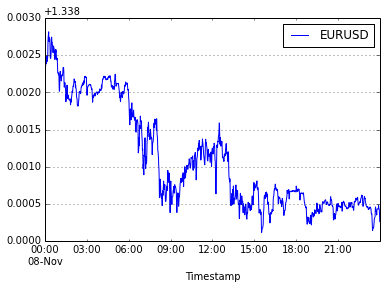
\includegraphics[width=0.8\textwidth]{img/euro_ppt}
                \caption{$EURUSD$}
                \label{fig:cpu_gpu_arch}
            \end{figure}
            \end{frame}
            \begin{frame}  
            \begin{figure}[h]
                \centering
                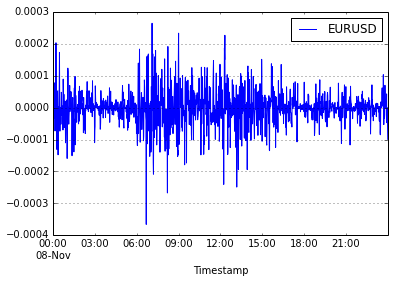
\includegraphics[width=0.8\textwidth]{img/euro_ppt_diff}
                \caption{$\Delta EURUSD$}
                \label{fig:cpu_gpu_arch}
            \end{figure}
            \end{frame}
                      
            \begin{frame}  
            \frametitle{Cointegración} 
            Definamos $\mathbf{Y}_t = \{\mathbf{y}^1, \dots, \mathbf{y}^l\}$
            como un set de $l$ series de tiempo estacionarias
            I(1) que se dice que es cointegrada si un vector,
            $\beta=[\beta(1),\dots,\beta(l)]^\intercal \in \mathbb{R}^l$  existe tal que la serie de tiempo,
            
            \begin{equation}
            \mathbf{Z}_t:= \beta^\intercal \mathbf{Y}_t = \beta(1) \mathbf{y}^1 + \dots + \beta(l) \mathbf{y}^l \sim
            \text{I(0)}
            \end{equation}
            
            En otras palabras, un set de variables I(1) se dice que son cointegradas si
            existe una combinación lineal de ellas que es I(0).
            \end{frame}
        
            \begin{frame}  
            \begin{figure}[h]
                \centering
                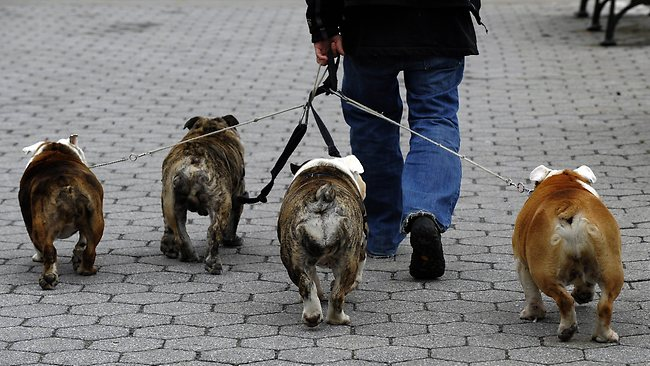
\includegraphics[width=0.8\textwidth]{img/dogs}
                \caption{Analogía borracho y los perros}
                \label{fig:cpu_gpu_arch}
            \end{figure}
            \end{frame}

        \subsection{Vector Autoregression}
            \begin{frame}
            \frametitle{Vector Autoregression}
            VAR describe el comportamiento de un set $l$ de
            variables endógenas como una combinación lineal de sus últimos $p$ valores.

            \begin{equation}
            \label{eq:variables}
            \mathbf{y}_t = 
            \begin{bmatrix} y_{1,t} \\
            y_{2,t} \\
            \vdots \\
            y_{l,t}
            \end{bmatrix}
            \end{equation}

            \begin{equation}
            \label{eq:var}
             \mathbf{y}_t = \phi_1 \mathbf{y}_{t-1}  + \dots +   \phi_p\mathbf{y}_{t-p}
             + \mathbf{c} + \mathbf{\epsilon}_t, \qquad t=p+1, \dots, N
             \end{equation}
            
            \noindent Donde $y_{j,t}$ corresponde a la serie de tiempo $j$ evaluada en el
            tiempo $t$.
            \end{frame}

            \begin{frame}
            La matriz VAR tiene la siguiente forma:
            \begin{equation}
             \label{eq:varmatrix}
             \resizebox{0.9\hsize}{!}{$%
                           \underbrace{ \begin{bmatrix}
                           \quad \\
                           \mathbf{y}_{p+1} &
                           \mathbf{y}_{p+2} &
                           \dots & 
                           \mathbf{y}_N \\
                           \quad
                           \end{bmatrix}}_{\substack{ \mathbf{B}\\l \times (N-p)}}   
            = 
                            \underbrace{\left[ 
                            \begin{array}{ccccc}
                            \quad & \quad & \quad & \quad & \quad \\
                            \phi_1  & \phi_2 & \cdots & \phi_p & \mathbf{c} \\  
                            \quad &\quad & \quad & \quad & \quad
                           \end{array} 
                           \right]}_{\substack{ \mathbf{X}\\ l \times (l \times p + 1 )}}
            \underbrace{\begin{bmatrix}
               \mathbf{y}_{p}  & \mathbf{y}_{p+1} & \dots    & \mathbf{y}_{N-1}\\
               \mathbf{y}_{p-1}  & \mathbf{y}_{p} & \dots    & \mathbf{y}_{N-2}\\
               \vdots        & \vdots   & \ddots   & \vdots\\
               \mathbf{y}_{1} & \mathbf{y}_{2}   & \dots    & \mathbf{y}_{N-p}\\
               1 & 1   & \dots    & 1 
               \end{bmatrix}}_{\substack{ \mathbf{A}\\ (l\times p +1 )(N-p)}}
            +
            \underbrace{\begin{bmatrix}
                            \quad \\
                          \mathbf{\epsilon}_{p+1}  & 
                          \mathbf{\epsilon}_{p+2}  & 
                          \dots                & 
                          \mathbf{\epsilon}_N \\
                          \quad
                         \end{bmatrix}}_{\substack{\mathbf{E}\\l \times (N-p) }} 
            $}
            \end{equation}
            \end{frame}
        \subsection{Vector Error Correction}
            \begin{frame}
            \frametitle{Vector Error Correction}
            El modelo VEC es una forma especial de un modelo VAR para variables I(1) que
            están también cointegradas. El modelo VEC es obtenido reemplazando
            $\Delta \mathbf{y}_t = \mathbf{y}_t - \mathbf{y}_{t-1}$ en ecuación
            (\ref{eq:var}). El modelo VEC es expresado en términos de diferencias,
            tiene un término de corrección de error y tiene la siguiente forma:
            
            \begin{equation}
             \label{eq:vec}
             \Delta \mathbf{y}_t = 
             \underbrace{ \Omega\mathbf{y}_{t-1}}_\text{Término de corrección de error} + 
             \sum_{i=1}^{p-1}
             \phi_i^* \Delta \mathbf{y}_{t-i}  + \mathbf{c} + \mathbf{\epsilon}_t \quad ,
            \end{equation}

            \end{frame}
            \begin{frame}
            Las matrices de coeficientes $\Omega$ y $\phi_i^*$ son
            funciones de matrices $\phi_i$ :
            
            \begin{eqnarray*}
            \phi_i^* &: =& -\sum_{j=i+1}^{p} \phi_j \\
            \Omega &: =& -(\mathbb{I}-\phi_1-\dots-\phi_p) 
            \end{eqnarray*}
            
            La matriz $\Omega$ tiene las siguientes propiedades:
            \begin{itemize}
            \item Si $\Omega = 0$ no hay cointegración
            \item Si $rank(\Omega)=l$ i.e full rank, entonces la serie de tiempo no es I(1)
            \item Si $rank(\Omega)=r,\quad 0 < r < l$ entonces, hay cointegración
            y la matriz $\Omega$ se puede expresar como $\Omega =
            \alpha \beta^\intercal$, donde $\alpha$ y $\beta$ son $(l \times r)$
            matrices y $rank(\alpha)=rank(\beta)=r$.
            \end{itemize}

            \end{frame}
            \begin{frame}
            Si existe cointegración, entonces la ecuación (\ref{eq:vec}) puede ser escrita:
            \begin{equation}
             \label{eq:vecfull}
              \Delta \mathbf{y}_t = \alpha \beta^\intercal\mathbf{y}_{t-1} 
               + \sum_{i=1}^{p-1} \phi_i^*\Delta
               \mathbf{y}_{t-i}  + \mathbf{c} + \mathbf{\epsilon}_t \quad ,
               \end{equation}
            
               \noindent que es un modelo VAR pero para series de tiempo diferenciadas.
            
            La forma matricial del modelo VEC es:
            \begin{equation} \label{eq:vecmatrix}
            \resizebox{0.9\hsize}{!}{$%
            \underbrace{
                            \left[ \begin{array}{ccc}
                           \quad & \mathbf{\Delta y}_{p+1} & \quad \\ 
                           \quad & \mathbf{\Delta y}_{p+2} & \quad \\
                           \quad & \vdots & \quad \\ 
                           \quad & \vdots & \quad \\  
                           \quad & \mathbf{\Delta y}_N & \quad 
                           \end{array} \right]}_{\substack{\mathbf{B}\\ (N-p) \times l }} =
               \underbrace{\left[ 
                \begin{array}{cccccc}
                 \quad & \quad & \quad & \quad & \quad & \quad \\
                 \alpha & \phi_1^*  & \phi_2^* & \cdots & \phi_{p-1}^* & \mathbf{c} \\  
                 \quad &\quad &\quad & \quad & \quad & \quad
                 \end{array} 
                  \right]}_{\substack{ \mathbf{X}\\ (l(p-1)+r+1) \times l}}
            \underbrace{\begin{bmatrix} 
               \beta^\intercal \mathbf{y}_{p} & 
               \beta^\intercal \mathbf{y}_{p+1}&
               \cdots & \beta^\intercal \mathbf{y}_{N-1} \\
               \mathbf{\Delta y}_p & \mathbf{\Delta y}_{p+1} & \cdots 
               & \mathbf{\Delta y}_{N-1} \\ 
               \vdots & \vdots & \ddots & \vdots \\
               \mathbf{\Delta y}_2 & \mathbf{\Delta y}_{3} & \cdots 
               & \mathbf{\Delta y}_{N-p+1} \\ 
               \end{bmatrix}}_{\substack{\mathbf{A} \\ (N-p) \times (l \times (p-1)+r+1) }}
            +
            \underbrace{\begin{bmatrix}
                          \quad &\mathbf{\epsilon}_{p+1} & \quad \\ 
                          \quad &\vdots & \quad\\ 
                          \quad & \vdots & \quad\\
                          \quad & \vdots & \quad\\
                          \quad &\mathbf{\epsilon}_N & \quad
                         \end{bmatrix}}_{\substack{\mathbf{E}\\ (N-p) \times l }} 
            $}
            \end{equation}

            \end{frame}
            %\begin{frame}
            %\end{frame}
        \subsection{Mínimos Cuadrados}
            \begin{frame}
            \frametitle{Mínimos Cuadrados}
            Consiste en minimizar la suma de los errores cuadrados que equivale
            a minimizar la siguiente expresión:
            
            \begin{equation}
            \label{eq:regressionproblem}
            \underset{\mathbf{X}}{\text{min}} \quad \| \mathbf{A}\mathbf{\mathbf{X}} - \mathbf{B} \|_2^2
            \end{equation}
            
            \noindent para la cual la solución conocida es $\hat{\mathbf{X}}$:
            
            \begin{equation}
            \label{eq:MP}
            \hat{\mathbf{X}}=\mathbf{A}^{\!\!+}\,\mathbf{B}
            \end{equation}
            
            \noindent donde $\mathbf{A}^{\!\!+}$ se puede escribir como:
            
            \begin{equation}
            \label{eq:pseudoinverse}
            \mathbf{A}^{\!\!+}= (\mathbf{A}^{\!\!\top} \mathbf{A})^{-1}\mathbf{A}^{\!\!\top} \, .
            \end{equation}

            \end{frame}
            \begin{frame}
            \frametitle{Algoritmo de Coleman}
            Este algoritmo resuelve el siguiente problema de optimización:
            
            \begin{equation}
            \label{eq:RRproblem}
            \underset{\mathbf{X}}{\text{min}} \quad \|
            \mathbf{A}\mathbf{\mathbf{X}} - \mathbf{B} \|_2^2 +\lambda \|
            \mathbf{\mathbf{X}}\|_2^2 
            \end{equation}
            
            \noindent donde $\lambda$ es un parámetro de regulación.
            
            La solución óptima $\mathbf{X}(\lambda)$ está determinada como:
            
            \begin{equation}
            \label{eq:optsolRR}
            \mathbf{X}(\lambda)=(\mathbf{A}^\top \mathbf{A}+ \lambda
            \mathbb{I})^{-1}\mathbf{A}^\top \mathbf{B} \, . 
            \end{equation}

            \end{frame}
	\section{GPU Computing}
        \begin{frame}
        \frametitle{CPU vs GPU}
        Las siglas GPU provienen de Graphics Processing Unit, o en español Unidad de
        procesamiento gráfico. Para efectos de hardware, la GPU funciona como
        coprocesador, pudiéndose utilizar de forma simultánea a la CPU y así aprovechar
        el potencial que puedan ofrecer ambas al mismo tiempo.

        \begin{figure}[h]
            \centering
            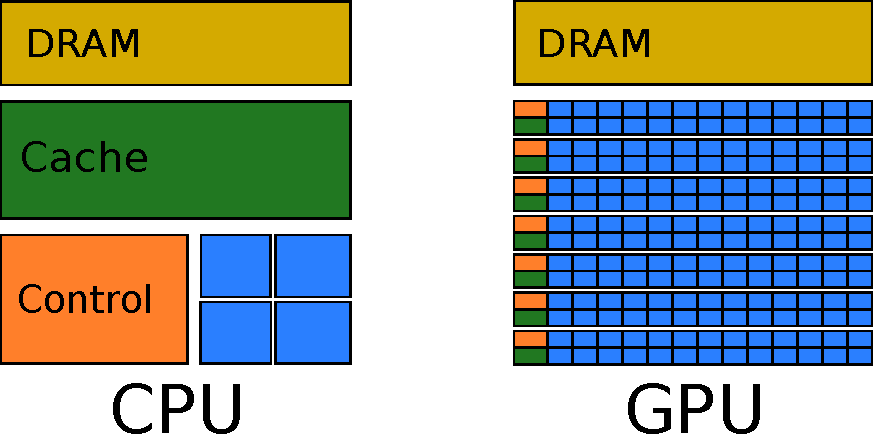
\includegraphics[width=0.6\textwidth]{img/cpu_gpu_arch.pdf}
            \caption{CPU y GPU vista general de su arquitectura}
            \label{fig:cpu_gpu_arch}
        \end{figure}
        \end{frame}

        \begin{frame}
        \frametitle{Lenguaje CUDA}
        CUDA como lenguaje de programación basado en la arquitectura 
        GPU y está sujeta a los elementos: \textbf{Thread/Hebras}, \textbf{Blocks/Bloques},
        \textbf{Grid/Malla}.
        
        \begin{figure}[h]
            \centering
            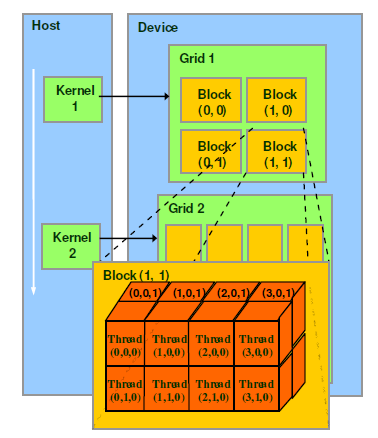
\includegraphics[height=0.5\textheight]{img/elements.png}
            \caption{CPU y GPU elementos generales}
            \label{fig:cpu_gpu_elements}
        \end{figure}
        \end{frame}

	\section{Metodología}
        \subsection{Algoritmo Propuesto}
            \begin{frame}
            \frametitle{Algoritmo Propuesto: Online VEC}
            Se propone un algoritmo online con ventanas deslizantes para la
            predicción del valor futuro de la cartera de stock FOREX usando el modelo
            VEC.
            \end{frame}

            \begin{frame}
            \begin{columns}[T] 
                \begin{column}{.58\textwidth}
                \begin{adjustbox}{max size={.95\textwidth}{.8\textheight}} %height=0.8\textheight}
                \begin{tikzpicture}[node distance=2cm]
                %\node (start) [startstop] {Start};
                %\node (in1) [io, below of=start] {Input};
                \node (in1) [io] {Input: y, p, L};
                \node (pro1) [process, below of=in1, yshift=-2.0cm] {$y_i = y[i:i+L]$ \\ 
                                                    $v = \texttt{Johansen}(\mathbf{y}_i,p)$ \\
                                                    $[\mathbf{A} \quad \mathbf{B}] =\texttt{vecm}(\mathbf{y}_i,p,v)$ \\
                                                    $\mathbf{X} = \text{OLS} (\mathbf{A},\mathbf{B})$  
                                                    $\mathbf{y}_{\text{true}}[i] = \mathbf{y}_i[-n,:]$ \\
                                                    $\mathbf{y}_{\text{pred}}[i] = \mathbf{A}[-n,:] \times \mathbf{X} +$ \\$ \mathbf{y}_i[-n-1,:-1]$ \\
                   };

                \node (pro2) [process, left of=pro1, xshift=-4cm] {$ i++ $}; 
               
                \node (dec1) [decision, below of=pro1, yshift=-2.5cm] { $i > it $ };
                
                \node (out1) [io, below of=dec1] {Output: $y_{true}, y_{pred}$};
                
                %\node (stop) [startstop, below of=out1] {Stop};
                
                %\draw [arrow] (start) -- (in1);
                \draw [arrow] (in1) -- (pro1);
                \draw [arrow] (pro1) -- (dec1);
                \draw [arrow] (dec1.west) -| node[anchor=east] {no} (pro2);
                \draw [arrow] (pro2) -- (pro1);
                \draw [arrow] (dec1) --  node[anchor=east] {si} (out1);
                %\draw [arrow] (out1) -- (stop);
                \end{tikzpicture}
                \end{adjustbox}
            \end{column}%

            \hfill%
            \begin{column}{.38\textwidth}
            Sliding Window VECM: SLVECM \\
            $\mathbf{y}$: Matriz con $N$ vectores de entrada y $l$ series de tiempo\\
            $p$: número de valores anteriores \\
            $L$: tamaño de la ventana deslizante ($L<N$) \\
            \end{column}%
            \end{columns}
            \end{frame}

            \begin{frame}
            \begin{columns}[T] 
                \begin{column}{.58\textwidth}
                \begin{adjustbox}{max size={.95\textwidth}{.8\textheight}} %height=0.8\textheight}
                \begin{tikzpicture}[node distance=2cm]
                %\node (start) [startstop] {Start};
                %\node (in1) [io, below of=start] {Input};
                \node (in1) [io] {Input: y, p, L, $\epsilon$, n};
                \node (pro1) [process, below of=in1] {$y_i = y[i:i+L]$};
                \node (dec1) [decision, below of=pro1, yshift=-0.5cm] {i = 0};
                \node (pro2a) [process, below of=dec1, yshift=-0.5cm] {$[\mathbf{A} \quad \mathbf{B}] =\texttt{ovecm}(\mathbf{y}_i,p,v,\mathbf{A},\mathbf{B})$
                                                                    $\Delta \mathbf{Y}_{\text{true}}[i] = \mathbf{B}[-1,:]$
                                                                    $\Delta \mathbf{Y}_{\text{pred}}[i] = \mathbf{A}[-1,:] \times \mathbf{X}$};

                \node (pro2b) [process, right of=dec1, xshift=4cm] {$v = \texttt{Johansen}(\mathbf{y}_i,p)$ $[\mathbf{A} \quad 
                                                                            \mathbf{B}] = \texttt{vecm}(\mathbf{y}_i,p,v)$};
                \node (pro3) [process, below of=pro2a, yshift=-0.5cm] {$\mathbf{X} = \text{OLS} (\mathbf{A},\mathbf{B})$ \\
                                                                    $\mathbf{y}_{\text{true}}[i] = \mathbf{y}_i[-n,:]$ \\
                                                                    $\mathbf{y}_{\text{pred}}[i] = \mathbf{A}[-n,:] \times \mathbf{X} +$ \\$ \mathbf{y}_i[-n-1,:-1]$ \\
                                                                    $e = \texttt{mape}(\mathbf{y}_{\text{true}}, \mathbf{y}_{\text{pred}})$};

                \node (dec2) [decision, below of=pro3, yshift=-0.5cm] { $e > \epsilon $ };

                \node (pro4a) [process, right of=dec2, xshift=4cm] {$v = \texttt{Johansen}(\mathbf{y}_i,p)$ \\
                                                                    $\mathbf{A} = \texttt{uvecm}(\mathbf{y}_i,p,v,\mathbf{A})$ \\
                                                                    $\mathbf{X} = \texttt{OLS} (\mathbf{A},\mathbf{B})$};

               
                \node (pro5) [process, left of=pro2a, xshift=-4cm] {$ i++ $}; 
               
                \node (dec3) [decision, below of=dec2, yshift=-0.5cm] { $i > it $ };
                
                \node (out1) [io, below of=dec3] {Output: $y_{true}, y_{pred}$};
                
                %\node (stop) [startstop, below of=out1] {Stop};
                
                %\draw [arrow] (start) -- (in1);
                \draw [arrow] (in1) -- (pro1);
                \draw [arrow] (pro1) -- (dec1);
                \draw [arrow] (dec1) -- node[anchor=east] {no} (pro2a);
                \draw [arrow] (dec1) -- node[anchor=south] {si} (pro2b);
                \draw [arrow] (pro2a) -- (pro3);
                \draw [arrow] (pro2b) |- (pro3);
                \draw [arrow] (pro3) -- (dec2);
                \draw [arrow] (dec2) --  node[anchor=south] {si} (pro4a);
                \draw [arrow] (pro4a) |- (dec3);
                
                \draw [arrow] (dec2) --  node[anchor=east] {no} (dec3);
                \draw [arrow] (dec3.west) -| node[anchor=east] {no} (pro5);
                \draw [arrow] (pro5) |- (pro1);
                \draw [arrow] (dec3) --  node[anchor=east] {si} (out1);
                %\draw [arrow] (out1) -- (stop);
                \end{tikzpicture}
                \end{adjustbox}
            \end{column}%

            \hfill%
            \begin{column}{.38\textwidth}
            Online VECM: OVECM \\
            $\mathbf{y}$: Matriz con $N$ vectores de entrada y $l$ series de tiempo\\
            $p$: número de valores anteriores \\
            $L$: tamaño de la ventana deslizante ($L<N$) \\
            $\epsilon$: MAPE umbral \\
            $n$: puntos de interpolación para calcular el MAPE\\
            \end{column}%
            \end{columns}
            \end{frame}

            %\begin{frame}
            %\frametitle{Parámetros del Algoritmo}
            %\begin{columns}[T] % align columns
            %\begin{column}{.48\textwidth}
            %\color{red}\rule{\linewidth}{4pt}
            %
            %Left Part
            %\end{column}%
            %\hfill%
            %\begin{column}{.48\textwidth}
            %\color{blue}\rule{\linewidth}{4pt}
            %
            %Right Part
            %\end{column}%
            %\end{columns}
            %\end{frame}
        \subsection{Diagrama de clases}
            \begin{frame}
            \frametitle{Diagrama de clases}
            \begin{columns}[T]
            \begin{column}{.48\textwidth}
            Python:
            \begin{itemize}
            \item Pandas
            \item Statsmodels
            \item Numpy
            \item Scikits.CUDA
            \end{itemize}
            \end{column}%

            \begin{column}{.48\textwidth}
            Clases:
            \begin{itemize}
             \item Util
             \item Reader
             \item Matrix
             \item Model
             \item ECM
             \item Model\_it
             \item Stats
            \end{itemize}
            \end{column}%
            \end{columns}
            \end{frame}

            \begin{frame}
            %\frametitle{Diagrama de clases}
            \begin{figure}[h!t]
                \begin{center}
                    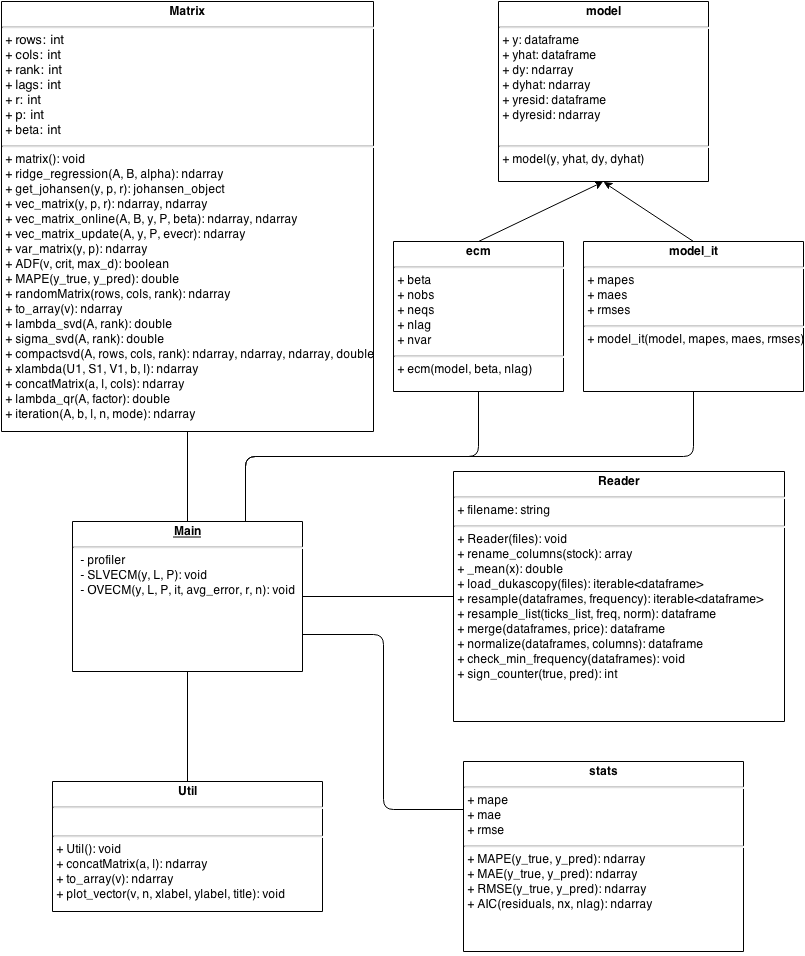
\includegraphics[width=0.8\textheight]{img/class_diagram.png}
                    \caption{Diagrama de Clases}
                    \label{fig:class_diagram}
                \end{center}
            \end{figure}

            \end{frame}
    \section{Experimentos}
        \subsection{Selección de data}
            \begin{frame}
            \frametitle{Selección de data} 
            \begin{figure}[h!t]
                \begin{center}
                    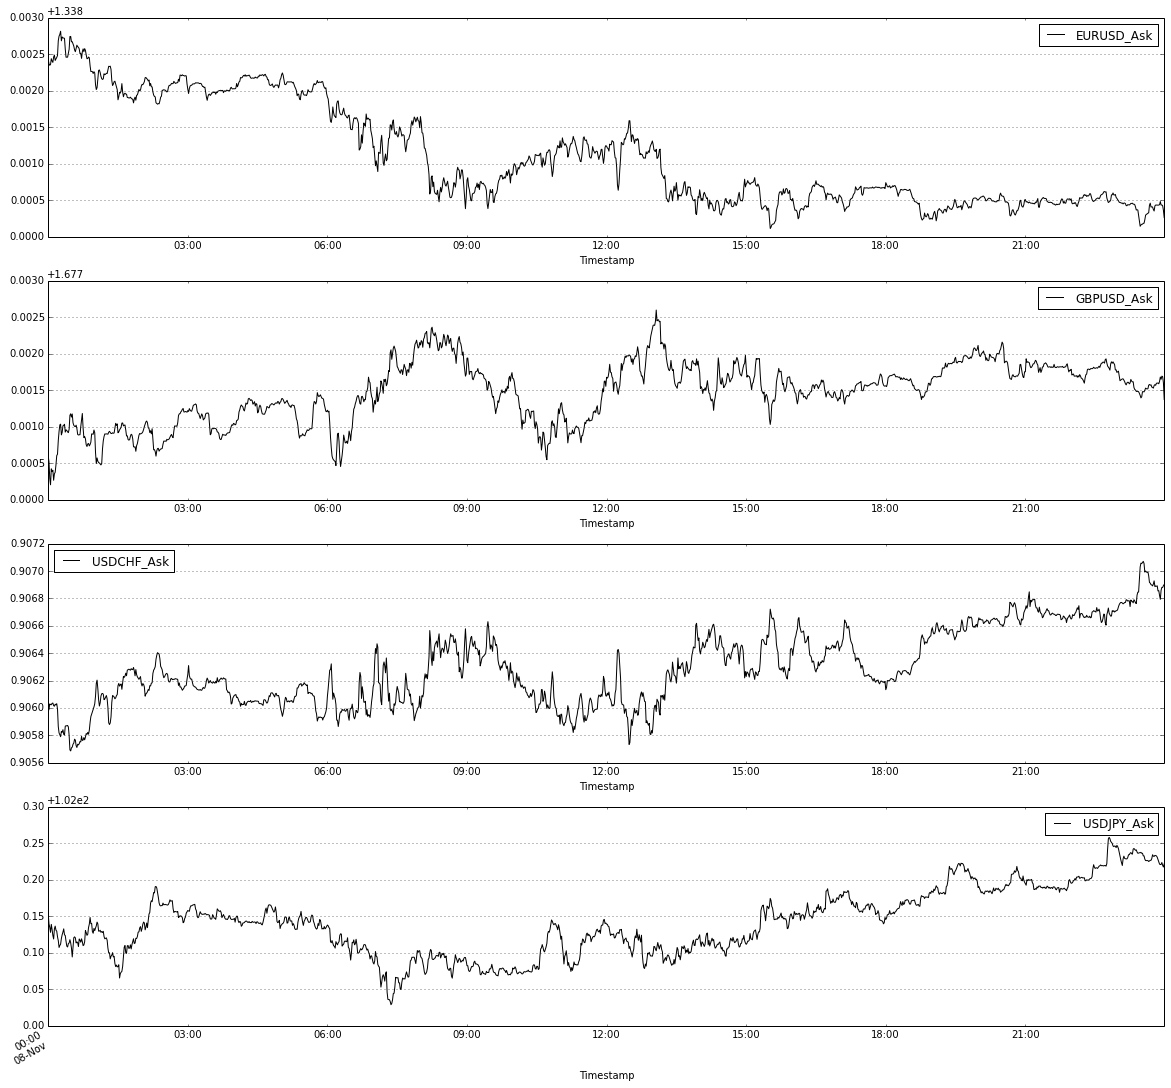
\includegraphics[width=0.8\textheight]{img/stocks_ask}
                    \caption{Precio Ask de las divisas}
                    \label{fig:stocks_ask}
                \end{center}
            \end{figure}
            \end{frame}

            \begin{frame}
            %\frametitle{}
            \begin{table}[h!]
            \caption{Data Tick}
            \label{tab:ticks}
            \begin{center}
            \begin{adjustbox}{max width=\textwidth}
            \begin{tabular}{|c|c|c|c|c|c|}
            \hline
            Date & Time & Ask & Bid& AskVolume & BidVolume \\
            \hline
            11-08-2014 & 00:00:00.000 & 1.34046 & 1.34042 & 1.25 & 1.69 \\
            11-08-2014 & 00:00:02.159 & 1.34047 & 1.34043 & 4.69 & 1 \\
            11-08-2014 & 00:00:02.667 & 1.34046 & 1.34042 & 1.32 & 2.44 \\
            11-08-2014 & 00:00:03.175 & 1.34046 & 1.34043 & 1.32 & 1 \\
            11-08-2014 & 00:00:07.058 & 1.34046 & 1.34043 & 3.75 & 1.69 \\
            11-08-2014 & 00:00:07.362 & 1.34043 & 1.34041 & 2.25 & 1 \\
            \hline
            \end{tabular}
            \end{adjustbox}
            \end{center}
            \end{table}
            \end{frame}
        %\subsection{Selección de Parámetros}
        %    \begin{frame}
        %    \frametitle{Selección de Parámetros}
        %    \begin{table}[h]
        %    \caption{Resultados de AIC}
        %    \label{tab:IAC}
        %    \begin{center}
        %    \begin{adjustbox}{max width=\textwidth}
        %    \begin{tabular}{|l|c|c|c|c|c|}
        %    \hline
        %    \backslashbox{\textbf{L}}{\textbf{P}} & \textbf{1} & \textbf{2} & \textbf{3} & \textbf{4} & \textbf{5} \\
        %    \hline
        %    100 & -58.64574 & \textbf{-58.83743} & -58.70088 & -58.61984 & -58.68117 \\
        %    400 & -60.42127 & -60.65667 & -60.67377 & -60.64634 &  \textbf{-60.68087} \\
        %    700 & -59.05503 & -59.17413 & \textbf{-59.20871} & -59.18571 & -59.17367 \\
        %    100 & -58.98121 & -59.09158 & \textbf{-59.12083} & -59.10099 & -59.0927 \\
        %    \hline
        %    \end{tabular}
        %    \end{adjustbox}
        %    \end{center}
        %    \end{table}
        %    \end{frame}
        \subsection{Pruebas de Cointegración}
            \begin{frame}
            \frametitle{Pruebas de Cointegración}
            \begin{figure}[h!t]
                \begin{center}
                    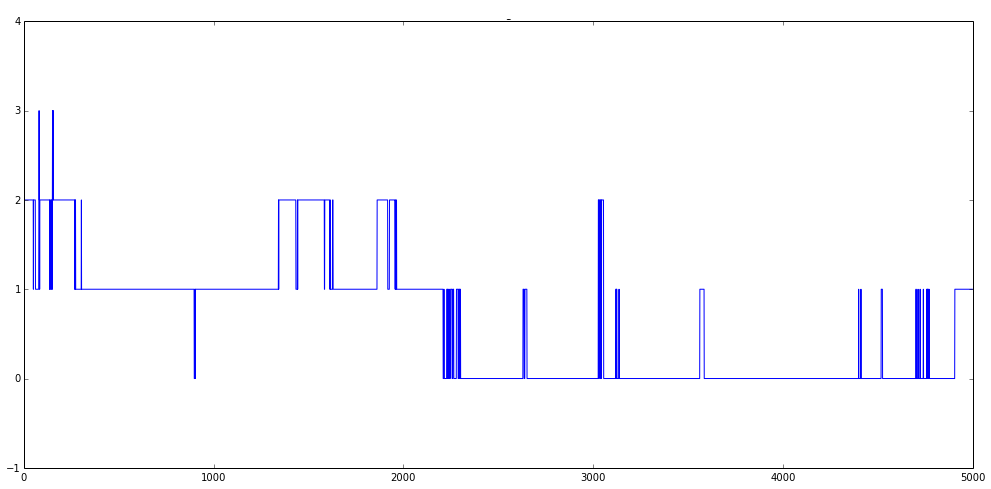
\includegraphics[width=0.8\textwidth]{img/betas}
                    \caption{Pruebas de Cointegración}
                    \label{fig:cointegracion}
                \end{center}
            \end{figure}

            \end{frame}
        \subsection{Test de raíz unitaria}
            \begin{frame}
            \frametitle{Test de raíz unitaria}
            \begin{table}[h!]
            \caption{Test de raíz unitaria, Frecuencia 60s}
            \label{tab:adf_60s}
            \begin{center}
            \begin{tabular}{|l|c|c|c|c|c|}
            \hline
            & \textbf{Estadístico} & \textbf{Valor Crítico} & \textbf{Resultado}\\
            \hline
            EURUSD          & -0.64 & -1.94 & True       \\
            $\Delta$ EURUSD & -70.45   & -1.94 & False       \\
            GBPUSD          & -0.63   & -1.94 & True          \\
            $\Delta$ GBPUSD & -54.53   & -1.94 & False       \\
            CHFUSD          & -0.88   & -1.94 & True         \\
            $\Delta$ CHFUSD & -98.98   & -1.94 & False       \\
            JPYUSD          & -0.65 & -1.94 & True        \\
            $\Delta$ JPYUSD & -85.78 & -1.94 & False     \\
            \hline
            \end{tabular}
            \end{center}
            \end{table}

            \end{frame}
        \subsection{Performance}
            \begin{frame}
            \frametitle{Performance - Online VECM}
            \begin{table}[h!]
            \caption{Tiempos de ejecución}
            \label{tab:extimes}
            \begin{center}
            \begin{tabular}{|l|c|c|c|c|c|}
            \hline
            & L & P & e  & Tiempo[s] \\
            \hline
            OVECM & 100 &p=2  & 0      & 2.492\\
            OVECM & 100 &p=2  & 0.0026  & 1.606\\
            SLVECM & 100 &p=2& -- & 2.100\\
            \hline
            OVECM & 400 & p=5  & 0      & 3.513\\
            OVECM & 400 &p=5  & 0.0041  & 2.569\\
            SLVECM & 400 & p=5 & -- & 3.222\\
            \hline
            OVECM & 700 &p=3  & 0      & 3.296\\
            OVECM & 700 &p=3  & 0.0032  & 2.856\\
            SLVECM & 700 &p=3 & -- & 3.581\\
            \hline
            OVECM & 1000 & p=3 & 0      & 4.387\\
            OVECM & 1000 & p=3  & 0.0022  & 2.408\\
            SLVECM & 1000 & p=3  & -- & 3.609\\
            \hline
            \end{tabular}
            \end{center}
            \end{table}
            \end{frame}

            \begin{frame}
            \frametitle{Algoritmo de Coleman}
            \begin{figure}[h!t]
                \begin{center}
                    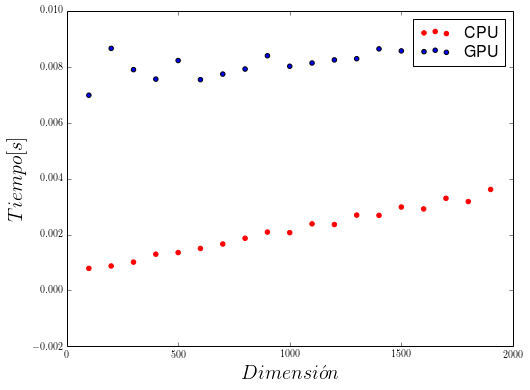
\includegraphics[width=0.7\textwidth]{img/speed_up_real}
                    \caption{Comparación tiempos de ejecución CPU y GPU, modelo real}
                    \label{fig:speedup_real}
                \end{center}
            \end{figure} 
            \end{frame}

            \begin{frame}
            %\frametitle{}
            \begin{figure}[h!t]
                \begin{center}
                    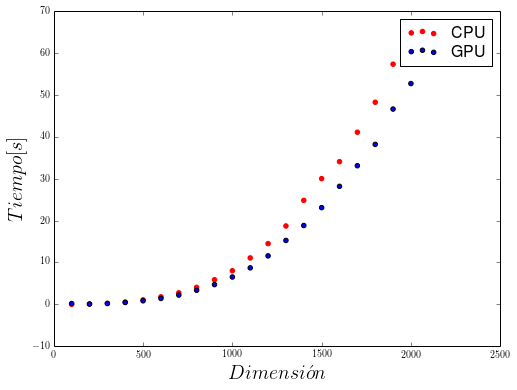
\includegraphics[width=0.7\textwidth]{img/speed_up_square}
                    \caption{Comparación tiempos de ejecución CPU y GPU, matrices cuadradas}
                    \label{fig:speedup_square}
                \end{center}
            \end{figure}
            \end{frame}

        \subsection{Resultados}
            \begin{frame}
            \frametitle{Resultados}
            \begin{table}[ht!]
            \caption{Métricas del modelo, Frecuencia 60s}
            \label{tab:mapes_60s}
            \begin{center}
            \begin{adjustbox}{max width=\textwidth}
            \begin{tabular}{|l|l|c|c|c|c|c|c|c|c|}
            \hline
            \multicolumn{4}{|c|}{Model} & \multicolumn{3}{|c|}{In-sample} &
            \multicolumn{3}{|c|}{Out-of-sample} \\
            \hline
            \hline
            Método & L & P & e &
            MAPE & MAE& RMSE&
            MAPE & MAE& RMSE \\
            \hline
             OVECM  &   100  &  P=2& 0.0026  &  0.00263&  0.00085&  0.00114&  0.00309&  0.00094&  0.00131\\
             OVECM  &   400  &  P=5& 0.0041  &  0.00378&  0.00095&  0.00127&  0.00419&  0.00103&  0.00143\\
             OVECM  &   700  &  P=3& 0.0032  &  0.00323&  0.00099&  0.00130&  0.00322&  0.00097&  0.00132\\
             OVECM  &   1000 &  P=3& 0.0022  &
             \textbf{0.00175}&  \textbf{0.00062}&  \textbf{0.00087} &
             \textbf{0.00172}&  \textbf{0.00061}&  \textbf{0.00090}\\
            \hline
             SLVECM  &   100 &  P=2& -  &  0.00262&  0.00085&  0.00113&  0.00310&  0.00095&  0.00132\\
             SLVECM  &   400 &  P=5& -  &  0.00375&  0.00095&  0.00126&  0.00419&  0.00103&  0.00143\\
             SLVECM  &   700 &  P=3& -  &  0.00324&  0.00099&  0.00130&  0.00322&  0.00098&  0.00132\\
             SLVECM  &   1000 &  P=3& -  &
             \textbf{0.00174}&  \textbf{0.00061}&  \textbf{0.00087}&
             \textbf{0.00172}&  \textbf{0.00061}&  \textbf{0.00090}\\
            \hline
            \end{tabular}
            \end{adjustbox}
            \end{center}
            \end{table}

            \end{frame}
    \section{Conclusiones}
            \begin{frame}
            \frametitle{Conclusiones}
            \begin{itemize}
            \item Cointegración
            \item OVECM vs SLVECM
            \item Mínimos Cuadrados
            \item Tiempo de ejecución
            \item Implementación
            \end{itemize}
            \end{frame}
        \subsection{Trabajo Futuro}
            \begin{frame}
            \frametitle{Trabajo Futuro}
            \newpage
            Finalmente y como trabajo futuro, se propone:
            \begin{itemize}
             \item Probar distintos métodos para la selección de parámetros. 
             \item Buscar cointegración de distintas monedas. 
             \item Incluir el volumen asociado al precio.
             \item Probar resultados con alguna estrategia. 
             \item Implementar el arribo de datos desde un servidor de datos. 
            \end{itemize}

            \end{frame}
    \frame{\titlepage}
\end{document}
